\documentclass{article}

\usepackage{amsmath}
\usepackage{graphicx}
\usepackage{hyperref}
\usepackage{tabularx}
\usepackage{xcolor}
\usepackage{float}


\title{Note on Tree of Thoughts: Deliberate Problem Solving with Large Language Models}

\begin{document}


\maketitle

\section{Motivation}

\textbf{Shortcoming} of current paradigm-original autoregressive mechanisms: Current LLMs 
fall short in tasks that require exploration, strategic lookahead, or where initial decisions 
play a pivotal role.

Analogous to the two modes of human thought, the simple associative token-level choices of 
LMs are reminiscent of "System 1"- a fast, automatic, unconscious mode. Thus might benefit from 
augmentation by a more delibrate "System 2" which can 

\begin{itemize}
    \item maintains and explores diverse alternatives for current choices instead of just picking one
    \item evaluates its current status and actively looks ahead or backtracks to make more global decisions
\end{itemize}

This paper the \textbf{Tree of Thoughts} (TOT) framework for general problem solving with LMs.

\begin{figure}[H]
    \centering
    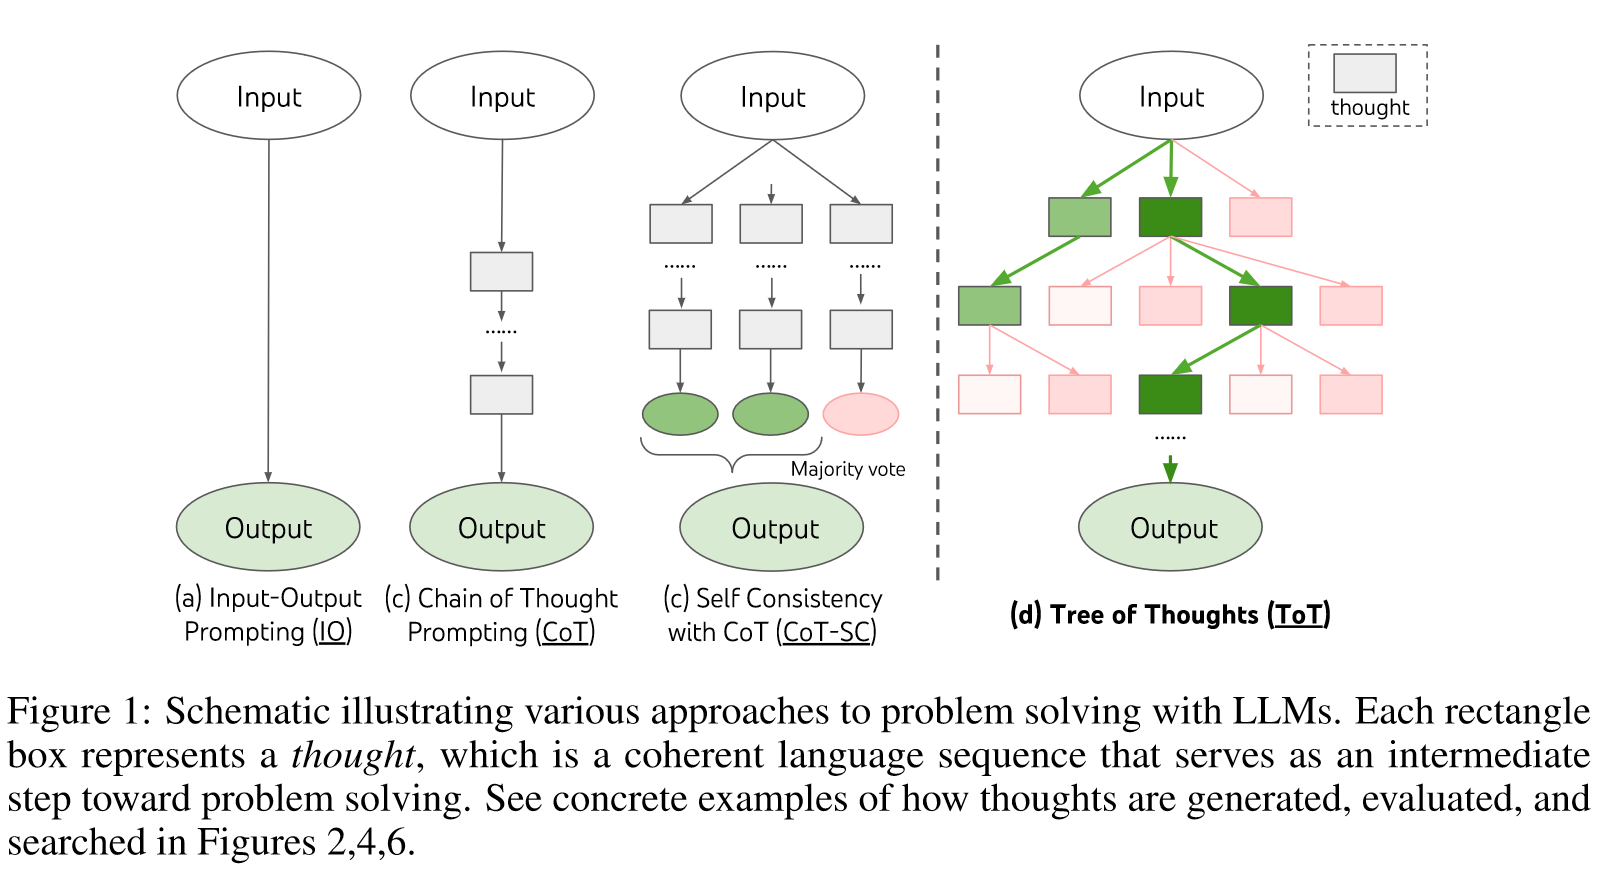
\includegraphics[width=\textwidth]{./Images/Figure1.png}
    \caption{Schematic illustrating various approaches to problem solving with LLMs. Each rectangle box represents a thought, which is a coherent language sequence that serves as an intermediate step toward problem solving.}
    \label{fig:Figure1}
\end{figure}

As Figure \ref{fig:Figure1} illustrates, while existing methods (detailed below) sample continuous language sequences for problem solving, ToT actively maintains a tree of thoughts, where each thought is a coherent language sequence that serves as an intermediate step toward problem solving (Table \ref{tab:Table1})

Finally, This paper combine this language-based capability to generate and evaluate diverse thoughts with search algorithms, such as breadth-first search (BFS) or depth-first search (DFS), which allow systematic exploration of the tree of thoughts with lookahead and backtracking.


\section{Background}




\begin{table}[h]
    \centering
    \begin{tabularx}{\textwidth}{|X|X|X|X|}
        \hline
        & \textbf{Game of 24} & \textbf{Creative Writing} & \textbf{5 $\times$ 5 Crosswords} \\
        \hline
        \textbf{Input} & 4 numbers \textcolor{blue}{(4 9 10 13)} & 4 random sentences & 10 clues \textcolor{blue}{(h1. presented;..)}\\
        \hline
        \textbf{Output} & An equation to reach 24\textcolor{blue}{(13-9)*(10-4)=24} & A passage of 4 paragraphs ending in the 4 sentences & 5x5 letters: \textcolor{blue}{SHOWN; WIRRA; AVAIL; ...} \\
        \hline
        \textbf{Thoughts} & 3 intermediate equations \textcolor{blue}{(13-9=4 (left 4,4,10); 10-4=6 (left 4,6); 4*6=24)} & A short writing plan \textcolor{blue}{(1. Introduce a book that connects...)} & Words to fill in for clues: \textcolor{blue}{(h1. shown; v5. naled; ...)} \\
        \hline
        \textbf{\#ToT steps} & 3 & 1 & 5-10 (variable) \\
        \hline
        \end{tabularx}

        \caption{Task overview. Input, output, thought examples are in blue}
        \label{tab:Table1}
\end{table}



\end{document}